\setchapterpreamble[u]{\margintoc}
\chapter{Energy System Modelling}
\labch{esm}


After completing this session successfully, you should be able

\begin{itemize}
\item to understand what a model is,
\item to understand the purpose of energy system models, and
\item to know about different characteristics of energy models.
\end{itemize}



\section{What are models?}
\labsec{models}


\paragraph*{Defining what a model is.}

\begin{kaobox}[frametitle=Task]
Have a look again at the task description for the homework of session 1 (Section \ref{sec:hw1}). How do you think the graph showing the future development was created?
\end{kaobox}


There are many different ways of defining what a model is. One widely used, general definition of a model has been developed by a researcher called Stachowiak \sidecite{stachowiak_allgemeine_1973}. He defines models by describing three important characteristics every model needs to fulfil. \refdef{model} lists all three characteristics.

\begin{definition}
\labdef{model}
Every model has three characteristics. A model
\begin{itemize}
\item  is always a model \textbf{of something}, i.e., it is a representation or depiction of a material or immaterial original,
\item is a simplification, i.e., does not have all attributes the original object has, and
\item aims to fulfil a particular purpose or function for the people building and/or using it.
\end{itemize}
\end{definition}

In short, a model is a simplified depiction of an original, built and used for a particular purpose. Such models can look very different and can have very different purposes. One example for a model is a physical miniature model of a building used by an architect to showcase the building design. The model is a depiction of an original building, either an existing building or a potential future building (characteristic 1). It is much smaller than the original and lacks a lot of the more detailed features, e.g., water pipes and furniture, and, thus, is a simplified representation of the original (characteristic 2). The model aims to fulfil a particular purpose, i.e., showcasing the architect's design to a project developer -- at the same time, it is inadequate to, for example, study the thermal performance of the original because it is built from very simple materials (characteristic 3). Another example would be a computer-based model of a chemical molecule that can be used by a chemist to predict the chemical properties of the molecule.


\paragraph*{Different kind of models.}~\\

Based on the definition from above, there is a wide range of different kind of models.

\begin{kaobox}[frametitle=Task]
Have a look at the pictures in \reffig{model_photos}. Which of those shows a) a model, b) an energy system model in particular, or c) no model at all? Explain your decisions.
\end{kaobox}

\begin{figure}[hb]
	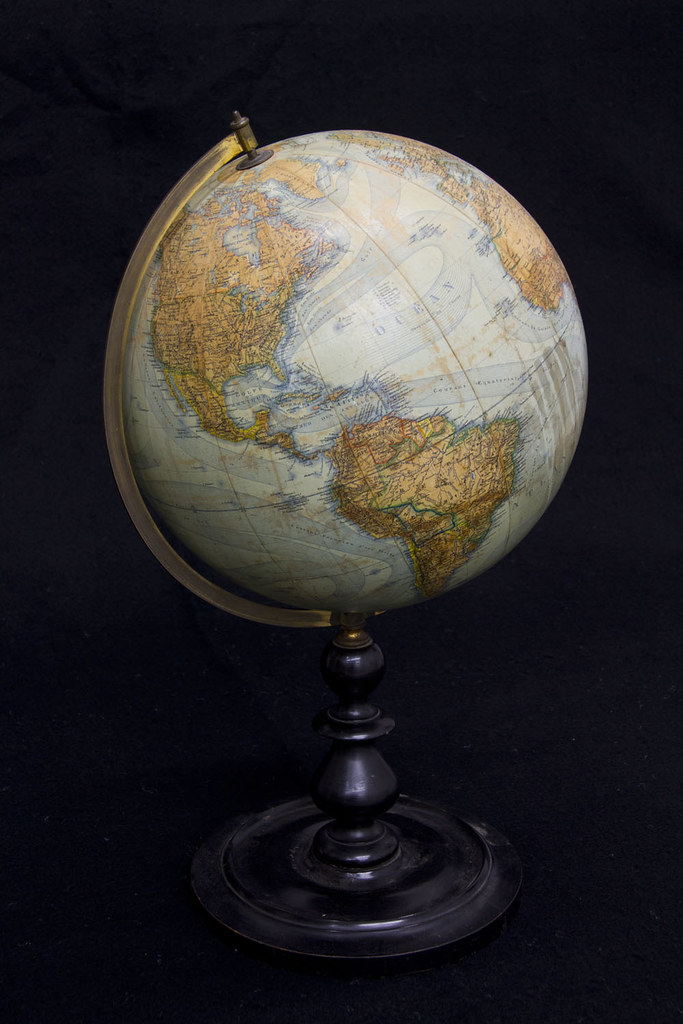
\includegraphics[height=0.38\textwidth]{files/Model_photo_1.jpg}
	
\includegraphics[height=0.38\textwidth]{files/Model_photo_2.jpg}\\
	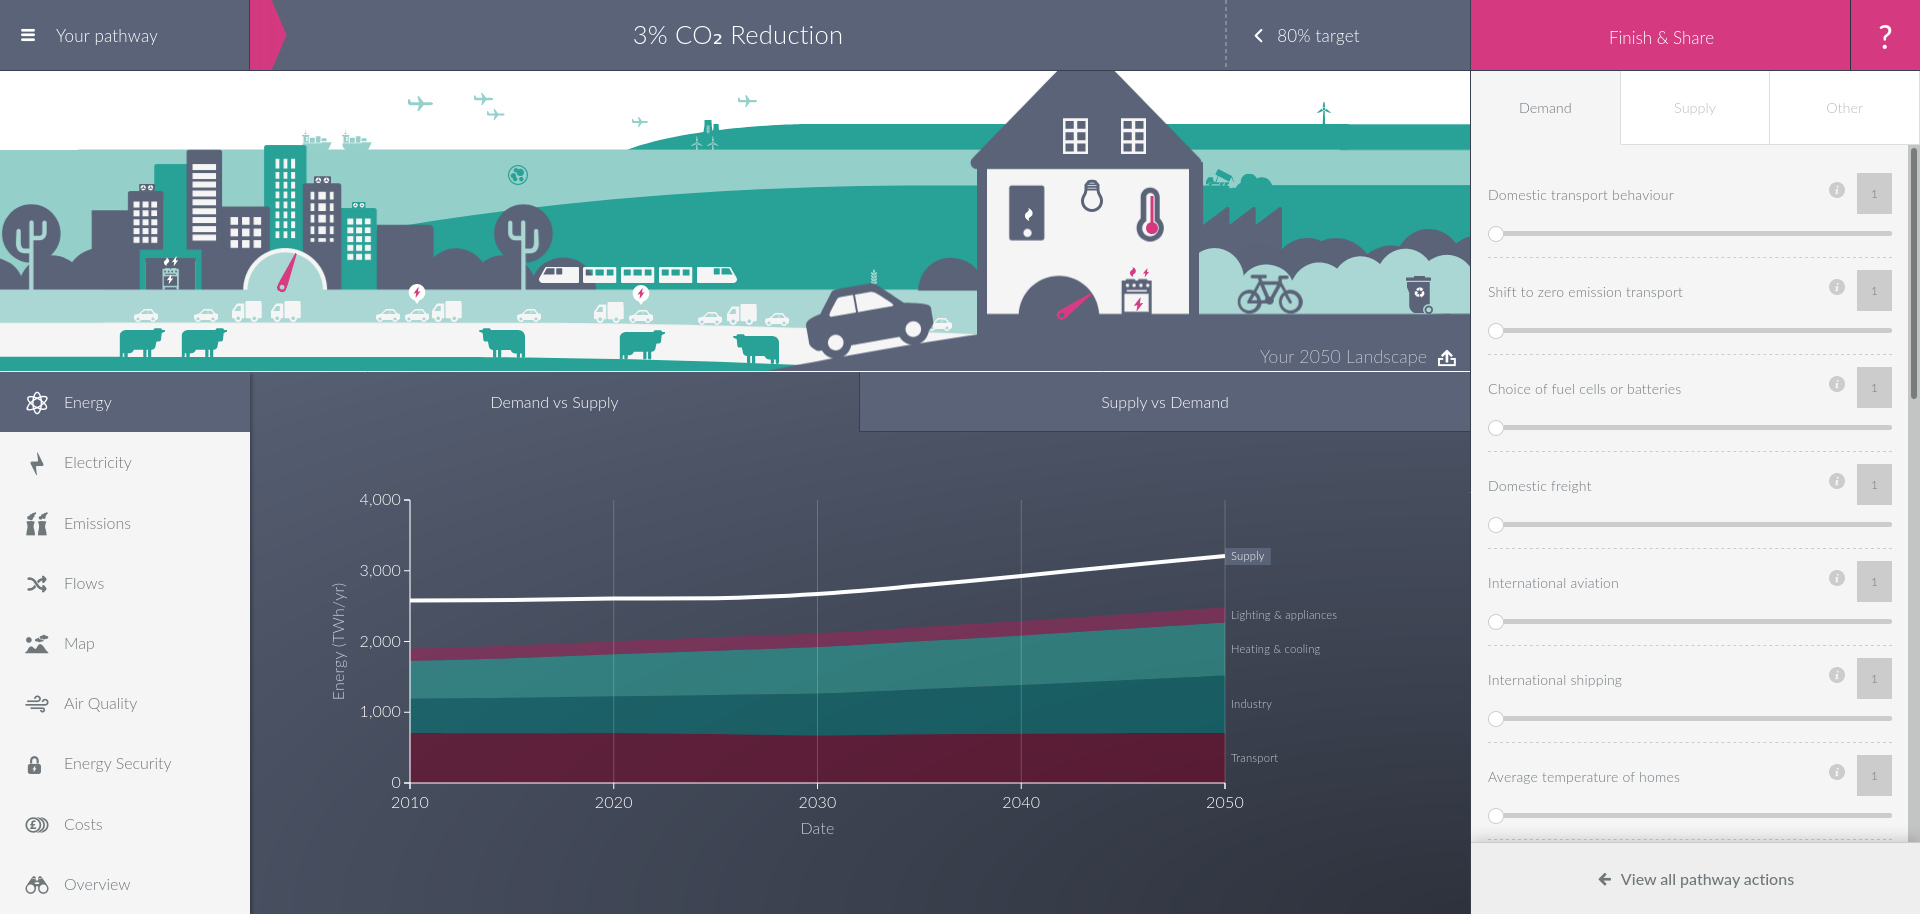
\includegraphics[height=0.24\textwidth]{files/Model_photo_3.png}
	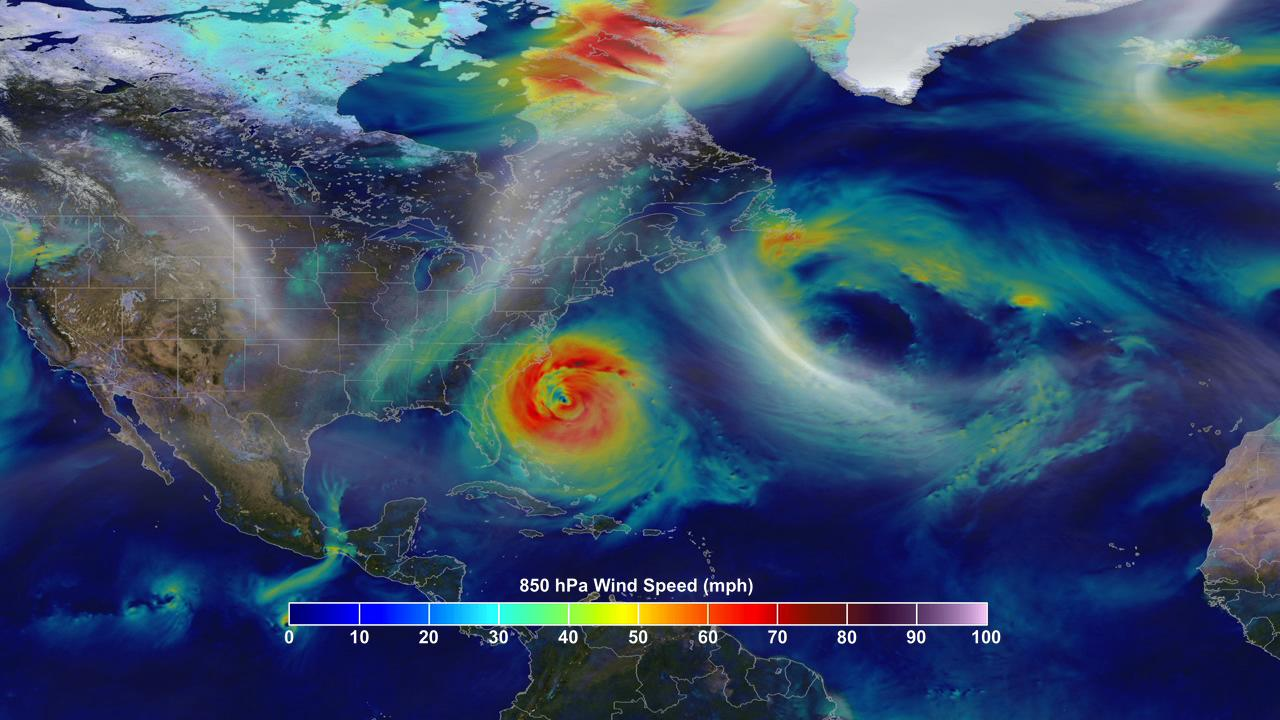
\includegraphics[height=0.24\textwidth]{files/Model_photo_4.jpg}
	\caption[Images showing different objects and/or models.]{Images showing different objects and/or models. Bottom left graphic, \copyright Leonhard Hofbauer, 2021, based on DECC released under a CC-BY-4.0, the remaining images, clockwise, are from LibraryArchives, Conal Gallagher, and NASA Goddard, respectively, and all licensed under a CC-BY-2.0}
	\labfig{model_photos}
\end{figure}

An \textbf{energy system model} is a model that depicts the energy system or at least parts of it. One could count some physical models, e.g., a small wind turbine model that is used to study design aspects, as energy model. Yet, this course focuses on computer-based energy system models that depict larger parts of the energy system (and are thus very difficult or impossible to build in a useful way as a physical model).

% TODO: add side note with more information on computer-based models

\section{The purpose of energy system models}


\paragraph{Energy models for energy planning.}~\\

Energy system models can have very different purposes but many of them are developed to support energy planning. Energy planning is the process of developing a plan with regard to the energy system for future years. Governments, companies, consumers, and many others all have to take decisions which rely on a plan for the energy future in one way or another. Have a look at the task below for one example.


\begin{kaobox}[frametitle=Task]
A local authority has to replace its entire fleet of diesel vans which are used as maintenance vehicles and for other council services. The vans can be separated in three different groups based on their usage profile. The table below  gives information about the number of vans in each group and the respective usage profile.


\begin{tabular}{ c c m{4cm} }
	\toprule
	Group & Number of vans & Distance driven per van and year (km)\\
	\midrule
	Maintenance vans & 10 & 25000\\
	Event vans & 8 & 8000 \\ 
	Other vans & 15 &20000  \\
	\bottomrule
\end{tabular}


The local council considers three different options for replacement of the fleet: the current type of diesel vans, electric vans, and biodiesel vans. The table below shows all the characteristics of the different types of vans.

\begin{tabular}{ c m{1.5cm} m{1.5cm} m{2cm} m{2cm} }
	\toprule
	Type & Capital cost (\pounds) & Lifetime (years) & Variable cost (incl. fuel) (\pounds /km)& CO$_2$ emissions (g/km)\\
	\midrule
	Diesel & 25000 & 20 &  0.08 & 300\\
	Electric & 35000 &  20 &  0.05 & 50 \\ 
	Biodiesel & 25000 & 20 &  0.10 & 100\\
	\bottomrule
\end{tabular}

How many vans of each type should the council buy if they want to minimize their annual cost but also reduce the annual CO$_{2}$ emissions from their fleet by at least 82\%? Work together in groups.\\
Tip: You can calculate the annual cost for a van in this simplified manner:\\
$ AnnualCost = CapitalCost/Lifetime + AnnualDistanceDriven \cdot VariableCost$.
\end{kaobox}

Energy planning can be a very complex task and involve questions which are very challenging to answer. Many of these questions cannot precisely be answered -- nobody knows for certain about the future -- but energy models can help us to get some answers and to think about the future in a structured way. They have been used to support decisions by the UK government, by companies, and by consumers. Because the energy system is very complex, ranging from local to global, from half-hourly to decade-long, no single model can answer all questions but many different ones are necessary to help different organisations with different energy planning questions.

% TODO: potentially add a table with different institutions, what decisions with regard to the energy system they need to take, and what underlying questions exist


\section{Different types of energy system models}

\paragraph{Differentiating energy system models.}~\\


As discussed earlier, there are a lot of different kind of energy system models with different purposes. \reftab{mclass} shows a few different characteristics we can look at when describing a particular model, along with a few potential values.~\\

% TODO: potentially add a definition of classification in a side note

\begin{table}[!t]
\caption[Classification of energy models.]{A number of different characteristics by which energy systems can be differentiated. Adapted from \cite{hall_review_2016}.}
\labtab{mclass}
\begin{tabular}{c c c }
\toprule
\bfseries Analytical approach  & \bfseries Methodology & \bfseries Sectoral coverage \\
\toprule
Top-Down  & Optimization & Whole energy system \\
Bottom-up & Simulation & Power sector  \\
Hybrid & Agent-based & Transport sector \\
Other& Econometric & Heat sector   \\
& ... & ... \\
\midrule
\bfseries Geographic coverage & \bfseries Time horizon &  \bfseries Time resolution\\
\midrule
Global &  Short term & Minute \\
National &  Medium term  & Hour \\
Regional &  Long term & Month\\
Local & & Year \\
... & & ...\\
\bottomrule
\end{tabular}
\end{table}

\begin{kaobox}[frametitle=Task]
In groups of three, come up with an energy planning question or problem and with what kind of model you could help to answer it:
\begin{itemize}
\item Think about one organization, e.g., the national government, a local authority, or a company, and what kind of question or problem they might face with regard to the future energy system. Write down the problem or question in 1-2 sentences.
\item Think about what kind of model might be appropriate to support the organization in their energy planning. You can use the classification in \reftab{mclass} to describe your model. Think about why you make your choices and note down the characteristics of your model.
\end{itemize}
Afterwards, your group needs to present your results, i.e., what organization you considered, what problem or question they might face, and what kind of model would be appropriate and why.
\end{kaobox}

    
\section{Homework}

% TODO: add more information about net-zero in a side note

In 2020, the UK government has published a simple, web-based energy model that can be used to explore pathways for the UK energy system towards its net-zero target in 2050. This is the successor of a similar tool called DECC 2050, which has been used widely by researchers, government, and other stakeholders.

The model (or calculator) has a normal and a detailed version which you can find here

\begin{itemize}
\item \href{https://my2050.beis.gov.uk/}{https://my2050.beis.gov.uk/} (normal)
\item \href{https://mackaycarboncalculator.beis.gov.uk/}{https://mackaycarboncalculator.beis.gov.uk/} (detailed)
\end{itemize}

Choose either the normal or detailed model and build a pathway that meets the government's net-zero target for 2050! Share your pathway with everybody through the virtual learning platform (once you are done creating your pathway, simply copy the current web address from the browser - it should look like this \textit{https://my2050.beis.gov.uk/?levers=1112 [...]} or this \textit{https://mackaycarboncalculator.beis.gov.uk/overview/emissions-and-primary-energy-consumption/?levers=1111 [...]}, depending on the calculator, and send it as a message to everyone) and have a look at the scenarios your classmates created. Be ready to discuss  your pathway and experience with the model in the next session.